\chapter{Detection and Reconstruction of Neutrinos in Ice} \label{chap:neutrino_detection}

This chapter explains the detection principle of the IceCube Neutrino Observatory as well as one of the reconstruction algorithms applied to extract information from the raw detector signals.
Section \ref{sec:icecube_deepcore} first presents the layout of IceCube and DeepCore before Section~\ref{sec:cherenkov_effect} and \ref{sec:energy_loss} explain the Cherenkov effect and the propagation of particles through ice.
Finally, Section~\ref{sec:event_reconstruction} outlines the reconstruction algorithm itself in detail.


\section{The IceCube Neutrino Observatory} \label{sec:icecube_deepcore}

\begin{figure}[ht]
	\centering
    \subfloat[IceCube Neutrino Observatory][Schematic sketch]{ \label{fig:icecube_array}
    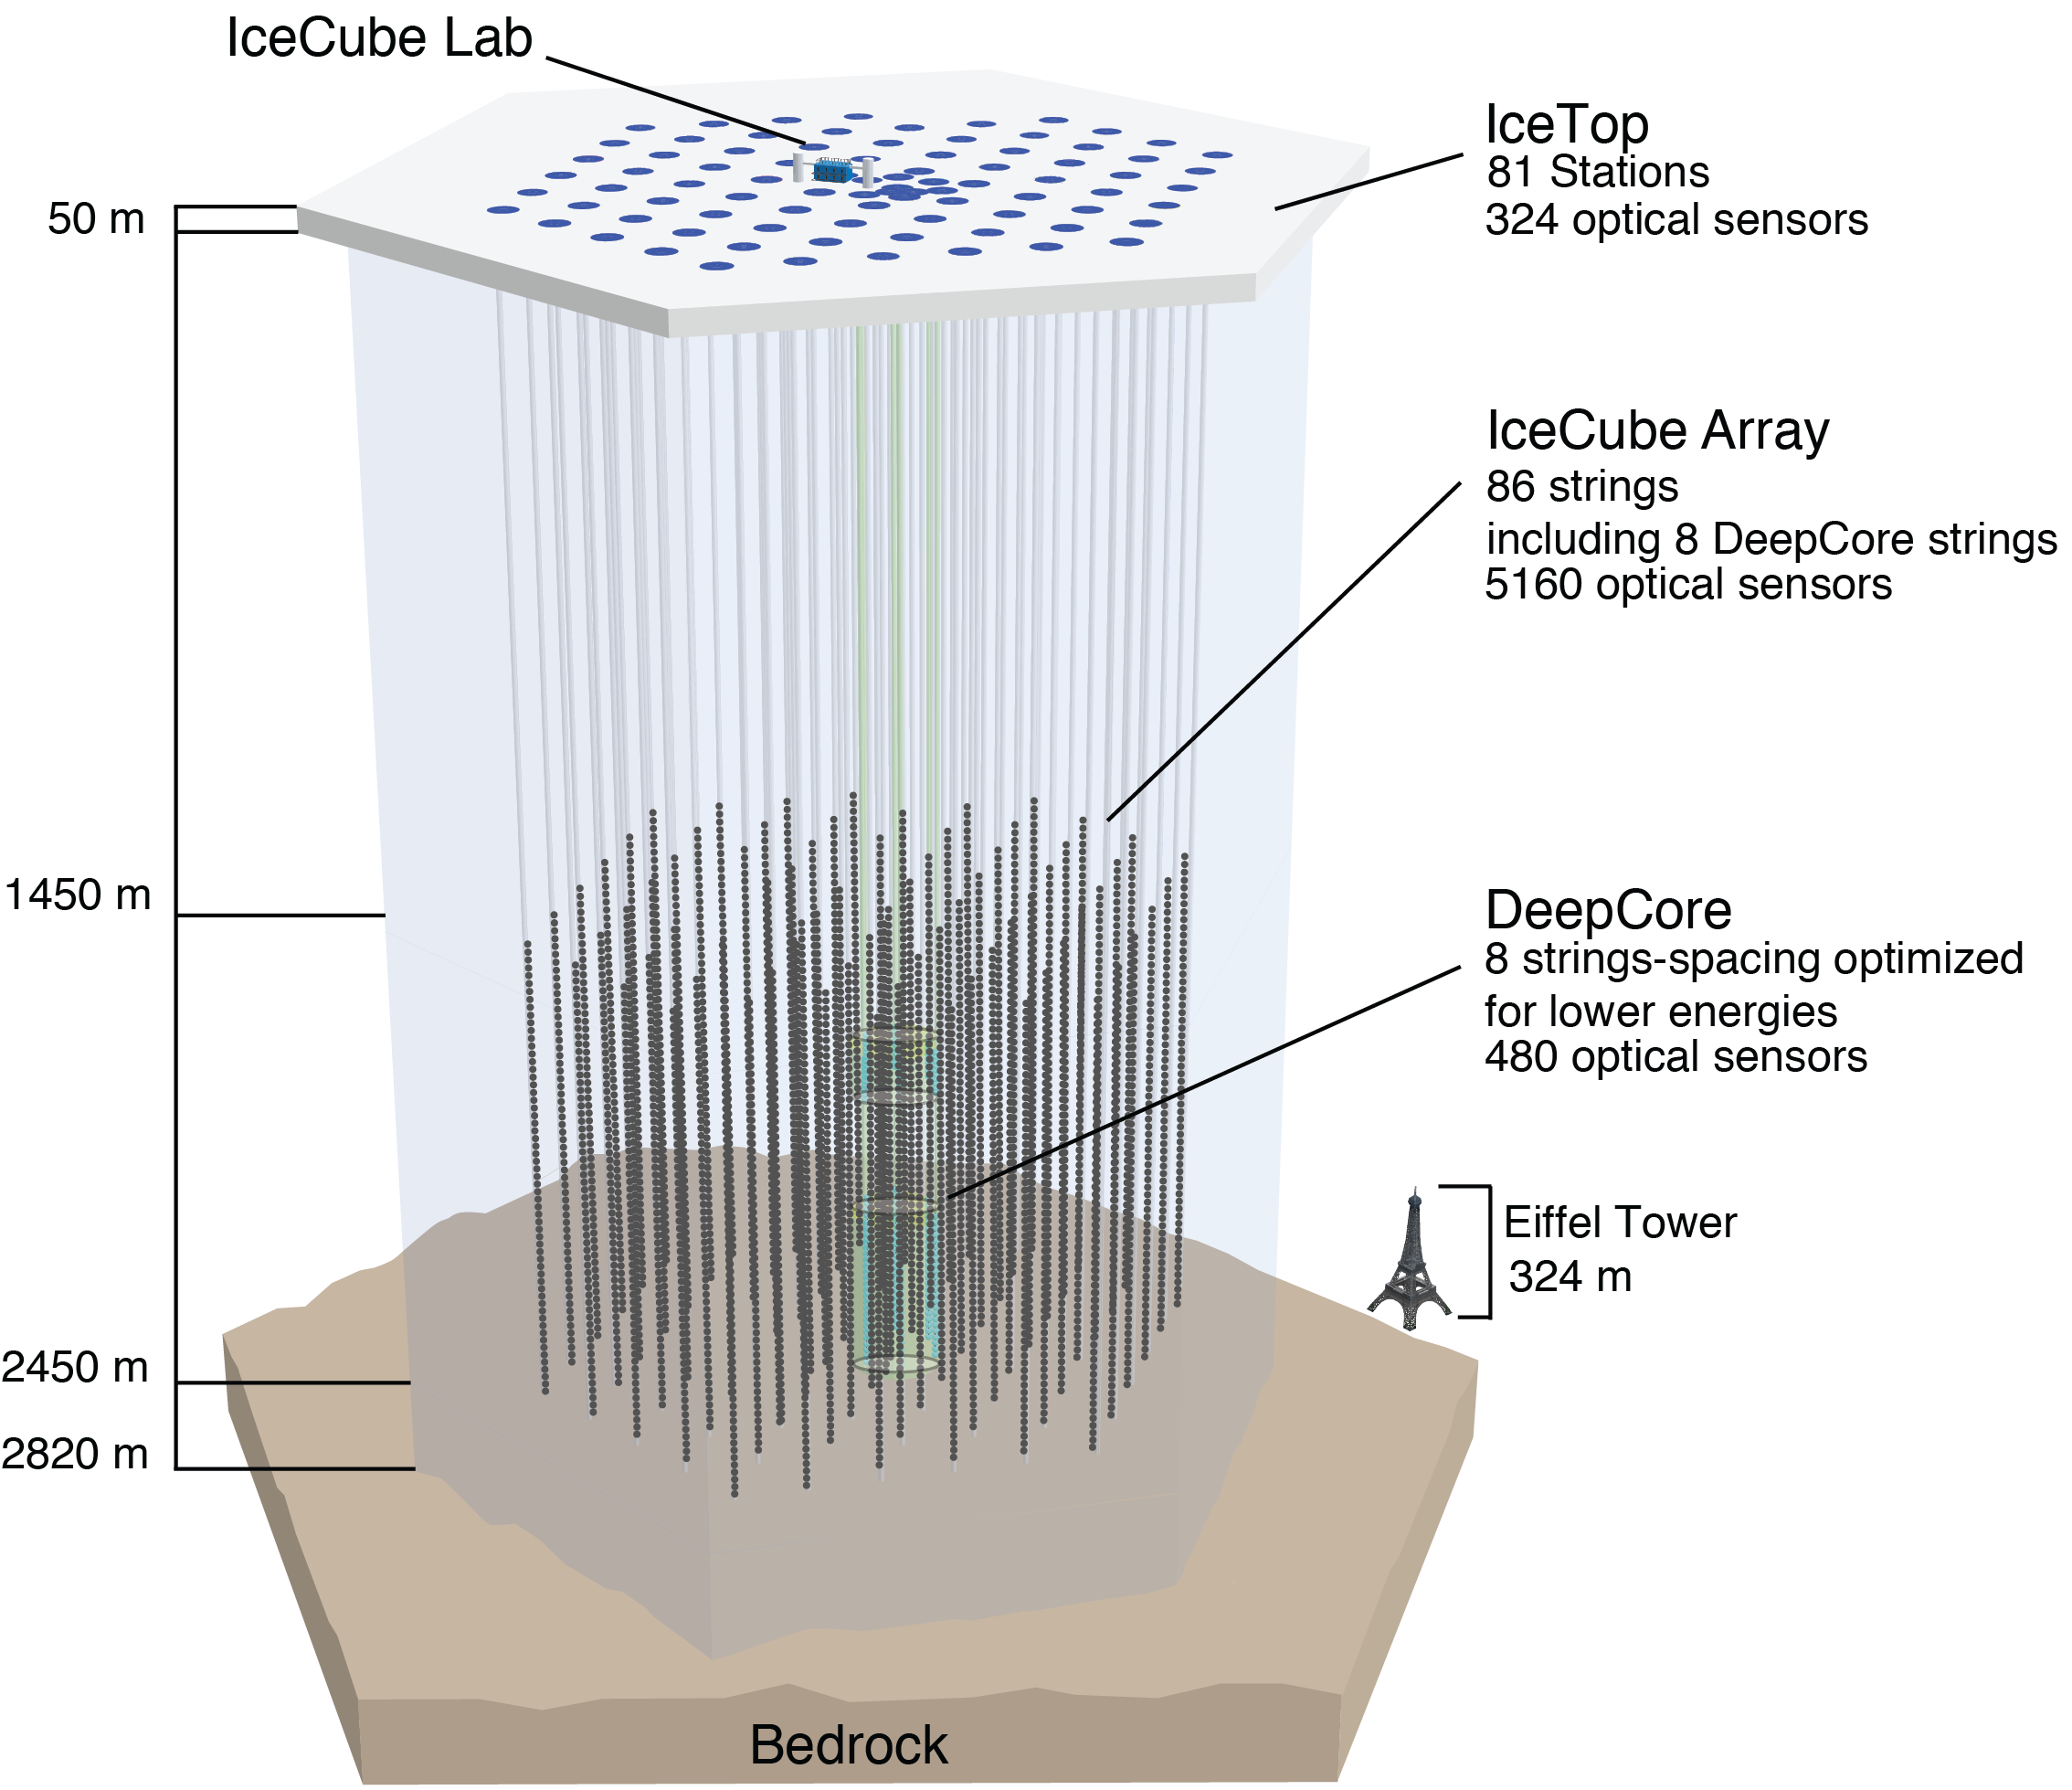
\includegraphics[align=b, width=0.55\linewidth]{figures/IceCubeArray_slim.png}
    }
    \subfloat[Digital Optical Module (DOM)][Design and components of a DOM]{ \label{fig:DOM_design}
    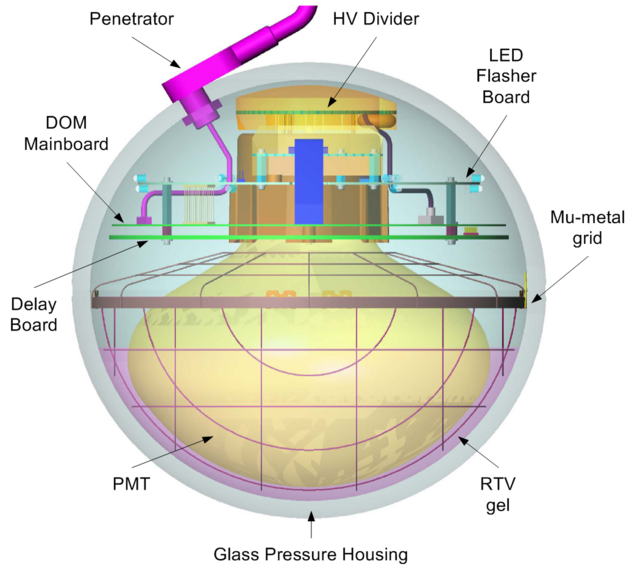
\includegraphics[align=b, width=0.4\linewidth]{figures/DOM_schematic.png}
    }
	\caption[IceCube Neutrino Observatory and Digital Optical Module]{The IceCube Neutrino Observatory and a schematic view of the Digital Optical Module (DOM). More detailed information can be found in \cite{2017JInst..12P3012A_Instrumentation_Systems}.}
\end{figure}

The IceCube Neutrino Observatory \cite{2017JInst..12P3012A_Instrumentation_Systems} is a cubic-kilometer particle detector located at the geographic south pole.
The detector consists of 86 vertical strings with 5160 optical sensors called digital optical modules (DOMs) \cite{ABBASI2009294_data_acquisition}.
Figure \ref{fig:icecube_array} shows a schematic overview of the detector layout with its main components.
The strings were drilled down into the Antarctic ice in a hexagonal arrangement shown in Figure~\ref{fig:icecube_top_view}.
60 optical sensors are placed on each string at depths of 1450-2450\,m below the ice.
IceCube is designed to detect neutrinos in the energy range $\mathcal{O}$(GeV)-$\mathcal{O}$(PeV).
Neutrinos can only be detected by the secondary charged particles created when they interact in the ice.
The optical sensors detect Cherenkov light produced by these charged particles (see Section~\ref{sec:cherenkov_effect}).
Using the observed light pattern, the neutrino energy, direction, and flavor can be reconstructed as described in Section~\ref{sec:event_reconstruction}.
The DOMs are made of a spherical glass housing containing a 10\," photomultiplier tube (PMT) in addition to the readout and processing electronics.
The modules are made to collect light, digitize the resulting PMT signal and send the data to the central data acquisition at the surface if a trigger condition is met.
The design of a DOM and its components is shown in Figure~\ref{fig:DOM_design}.

\begin{figure}[h]
    \begin{center}
        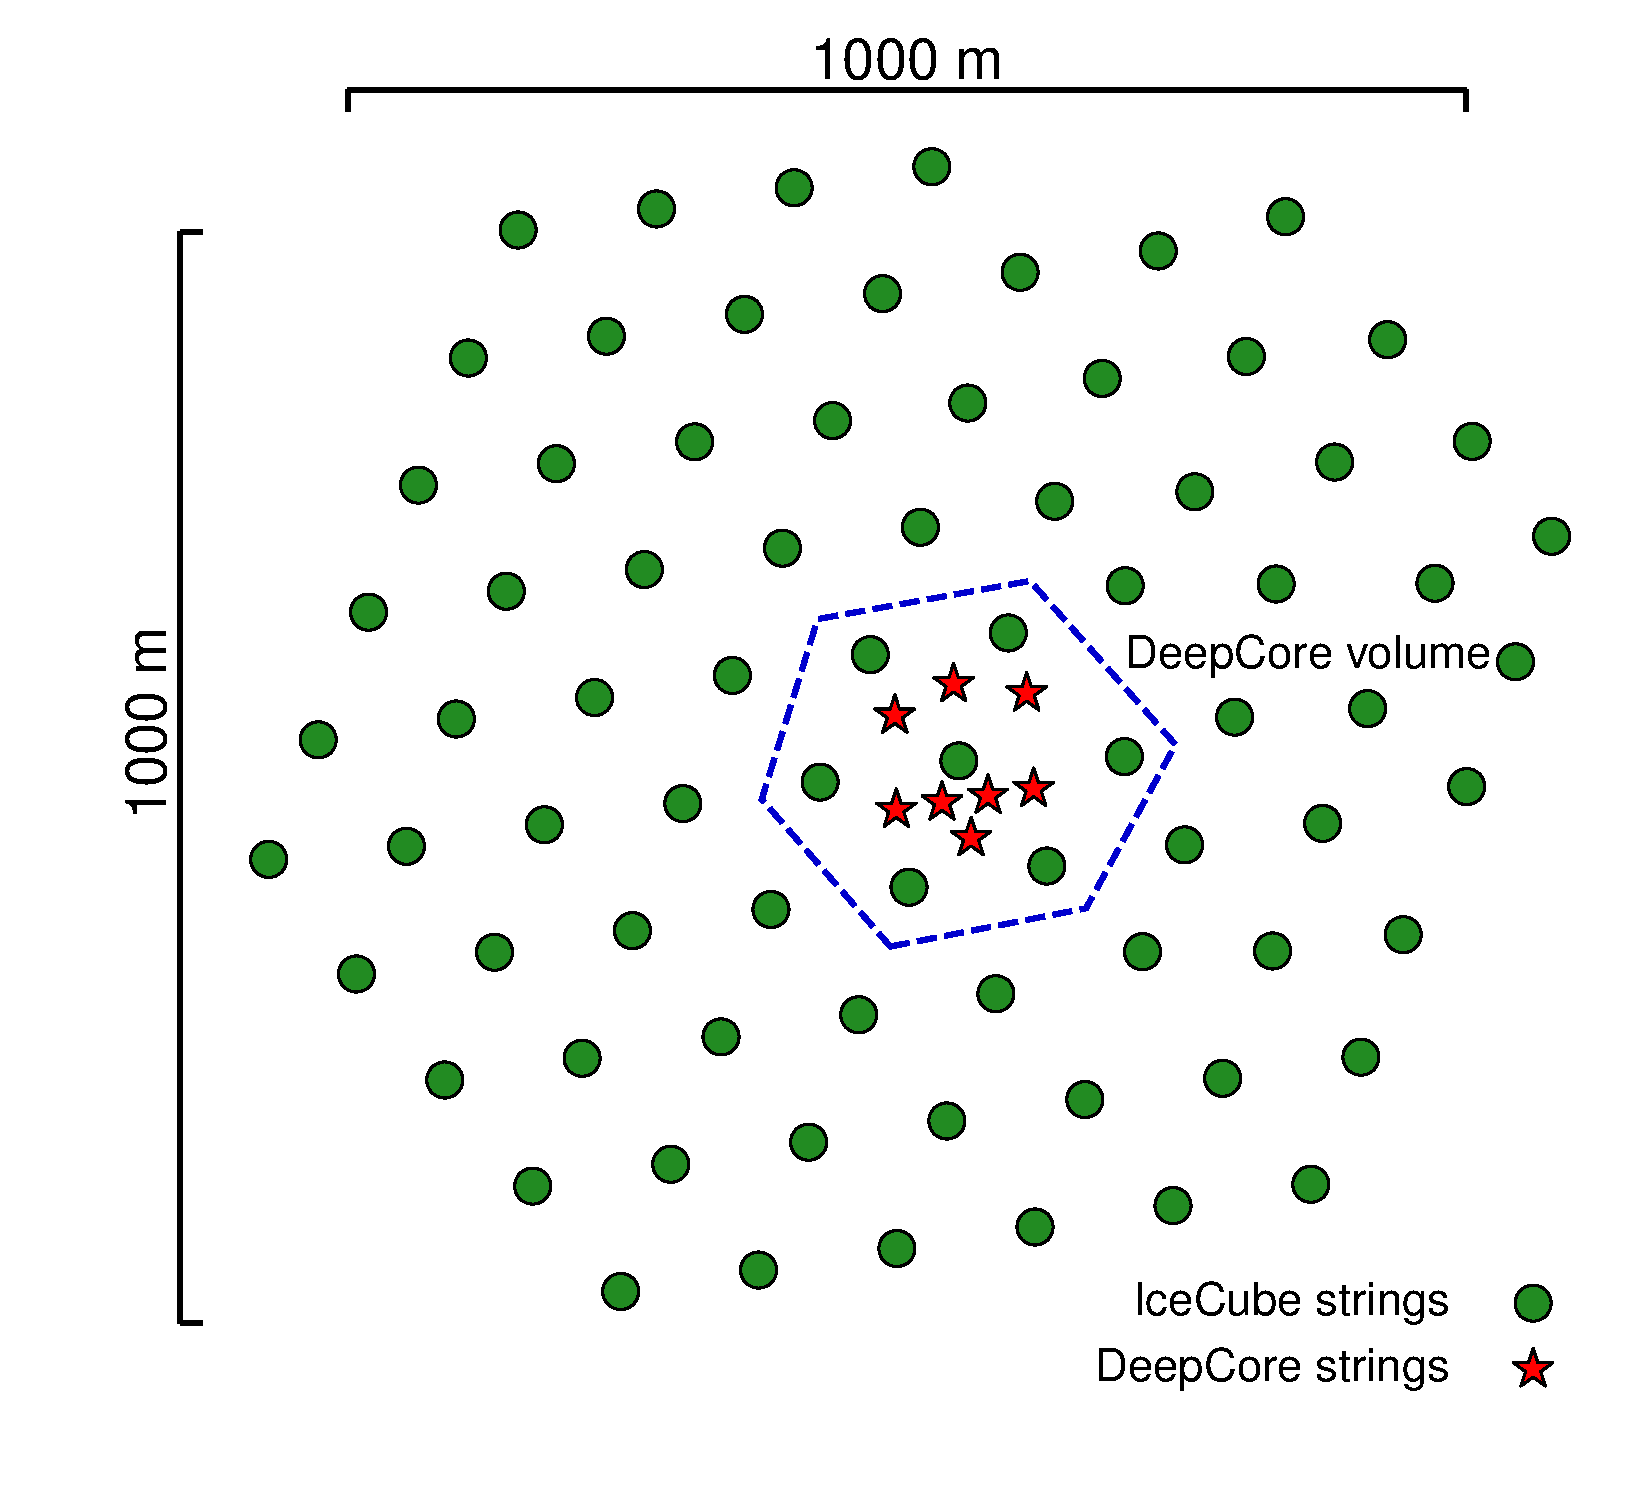
\includegraphics[trim={2.0cm, 1.5cm, 0, 0}, clip, width=0.65\linewidth]{figures/icecube_top_view_bw.pdf}
    \end{center}
    \caption[IceCube top view]{Top view of the IceCube array.}
    \label{fig:icecube_top_view}
\end{figure}

The main part of IceCube is formed by 78 strings with 125\,m horizontal spacing and 17\,m vertical spacing between DOMs.
This results in a neutrino detection energy threshold of 100\,GeV. There are 8 additional strings that form a denser sub-array of IceCube called DeepCore \cite{DeepCore_design_Abbasi2012615}.
DeepCore is at the bottom-center of the detector and includes these 8 strings as well as the 7 surrounding IceCube strings in the fiducial volume shown in Figure~\ref{fig:icecube_top_view}.
The strings in this volume have an average distance of about 70\,m.
The majority of the DeepCore DOMs are placed between 2100\,m and 2450\,m below the ice and the vertical spacing is 7\,m.
Around 2050\,m there is a dust layer with bad optical properties. Above the dust layer, there are a few additional DeepCore modules used as a veto cap.
The denser spacing and the application of high quantum efficiency DOMs in DeepCore as well as the fact that the ice between 2100\,m and 2450\,m has the best optical properties leads to a lowered neutrino detection energy threshold of around 5\,GeV.
DeepCore is optimized for the observation of neutrinos in the energy range of $10-100$\,GeV.
This is the energy range where the oscillation signal from atmospheric neutrinos can be observed and studied.
The surrounding IceCube strings and the veto cap are used to reject atmospheric muons that are the main background in neutrino oscillation measurements.

The coordinate system \cite{2017JInst..12P3012A_Instrumentation_Systems} used in IceCube is centered at 46500'E, 52200'N at an elevation of 883.9\,m.
It is defined as a right-handed coordinate system with the y-axis pointing along the Prime Meridian (Grid North) towards Greenwich, UK and the x-axis pointing 90\,degrees clockwise from the y-axis (Grid East).
The z-axis is normal to the  Earth's surface, pointing away from the surface.
Additionally, the depth in IceCube is defined as the vertical distance from the ice surface, set to be at an elevation of 2832\,m.


\section{Cherenkov Effect} \label{sec:cherenkov_effect}

Cherenkov radiation is emitted when a charged particle moves through a medium with a velocity that is greater than the speed of light in that medium.
The continuous energy loss due to the emission of Cherenkov radiation is small, at the order of $\mathcal{O}$($10^{-4}$), as compared to the main energy losses that will be described in Section~\ref{sec:energy_loss}.
The observation of this radiation in IceCube and DeepCore, however, is fundamental for the detection of the charged particles originating from the neutrino interactions that were outlined in Section~\ref{sec:neutrino_interactions}.
The Cherenkov effect was first observed by Pavel Cherenkov in 1934 \cite{CherenkovPhysRev.52.378}.
As can be derived from trigonometry, the Cherenkov light is emitted in a parallel wavefront at the Cherenkov angle
\begin{equation}
    \theta_c = \arccos\Big(\frac{1}{\beta n}\Big),
    \label{eq:cherenkov_angle}
\end{equation}
with $n$ being the refractive index of the medium and $\beta$ the speed of the particle in units of the speed of light.
A sketch of the wavefront is shown in Figure~\ref{fig:cherenkov_light_front}, where the black circles depict spherically emitted light and the blue line is the formed Cherenkov light front.
\begin{figure}[h]
    \centering
    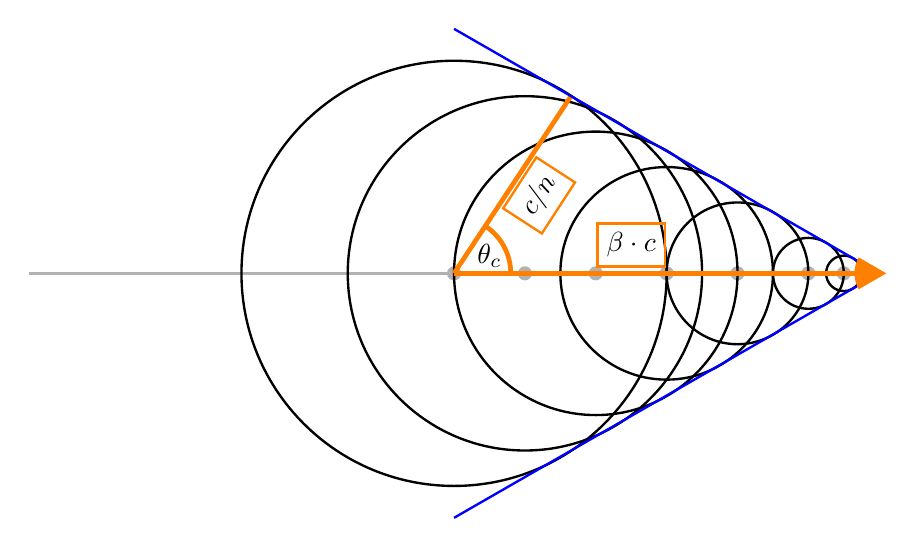
\begin{tikzpicture}[scale=0.9]
        \draw[draw=none,fill=gray!60] (8,0) circle (0.1);
        \draw[draw=none,fill=gray!60] (9,0) circle (0.1);
        \draw[draw=none,fill=gray!60] (10,0) circle (0.1);
        \draw[draw=none,fill=gray!60] (11,0) circle (0.1);
        \draw[draw=none,fill=gray!60] (12,0) circle (0.1);
        \draw[draw=none,fill=gray!60] (13,0) circle (0.1);
        \draw[draw=none,fill=gray!60] (13.5,0) circle (0.1);
        
        \draw[line width=0.3mm, gray!60] (2,0)--(14,0);
        
        \draw[line width=0.3mm] (8,0) circle (3);
        \draw[line width=0.3mm] (9,0) circle (2.5);
        \draw[line width=0.3mm] (10,0) circle (2);
        \draw[line width=0.3mm] (11,0) circle (1.5);
        \draw[line width=0.3mm] (12,0) circle (1);
        \draw[line width=0.3mm] (13,0) circle (0.5);
        \draw[line width=0.3mm] (13.5,0) circle (0.25);
        
        \draw[orange, line width=0.6mm] (8,0)--(14,0);
        \draw[orange, line width=0.6mm] (8,0)--(9.65,2.5);
        
        \draw[orange, line width=0.6mm] (8.8,0) arc (0:55:0.8cm);
        
        \draw[blue, line width=0.3mm] (8,3.45) -- (14,0);
        \draw[blue, line width=0.3mm] (8,-3.45) -- (14,0);
        
        \draw[draw=none,fill=orange] (14.1,0)-- +(210:0.45cm)arc (210:150:0.45cm) -- cycle;
        
        \node[] at (8.5,0.25) {$\theta_c$};

        \node[draw=orange,line width=0.3mm] at (10.5,0.4) {$\beta \cdot c$};
        \node[draw=orange,line width=0.3mm,, rotate=57] at (9.2,1.1) {$c/n$};
    \end{tikzpicture}
    \caption[Cherenkov light front]{Schematic formation of the Cherenkov light front (blue) produced by a charged particle traveling faster than the speed of light in the medium. The black circles are spherically emitted light and the orange arrow shows the direction of the particle.}
    \label{fig:cherenkov_light_front}
\end{figure}
Typical values for the Antarctic ice are $n \approx 1.3$ and as a result $\theta_c \approx 41^\circ$ \cite{SEuler}.
Additionally, one can calculate the number of photons produced by a Cherenkov emitter based on the description in \cite{Frank_Tamm}.
For a wavelength $\lambda$ with (300\,nm < $\lambda$ < 500\,nm) 250 photons per cm are emitted assuming a very relativistic particle with $\beta \simeq 1$ \cite{raedel_wiebusch_cherenkov_yield}.


\section{Energy Losses} \label{sec:energy_loss}

When charged particles travel through matter they interact and lose energy by several interaction processes.
The Cherenkov light emitted by the particles as described in Section~\ref{sec:cherenkov_effect} only contributes a small amount to the total energy loss.
The dominant processes depend on the type of Cherenkov light source, which we can broadly categorize into the three groups: quasi-continuous energy loss by muons, electromagnetic cascades, and hadronic cascades.

\paragraph{Muons} lose their energy mainly by \textit{ionization}, \textit{bremsstrahlung}, \textit{pair production} and the \textit{photo-nuclear interaction}.
Considering that ionization only has a weak energy dependence for muons above 1\,GeV and combining the other three components into one, the total energy loss is given by
\begin{equation}
    -\frac{\mathrm{d}E}{\mathrm{d}x} = a_I(E) + b_R(E) \cdot E,
    \label{eq:radiative_losses}
\end{equation}
where $E$ is the energy and $a_I(E)$ and $b_R(E) \cdot E$ are the energy loss by ionization and the combined radiative losses, respectively.
For the energy range of interest for this work, the parameters $a_I(E)$ and $b_R(E)$ only have a weak energy dependence and equation \ref{eq:radiative_losses} reduces to
\begin{equation}
    -\frac{\mathrm{d}E}{\mathrm{d}x} = a + b \cdot E.
    \label{eq:radiative_losses_simple}
\end{equation}
This description results in a critical energy $E_{crit}=a/b$ separating the two energy regimes where ionization or radiative losses are dominant.
Typical values are $a \approx 2.59$\,MeV/cm and $b \approx 3.63 \cdot 10^{-6}$\,cm$^{-1}$ \cite{2004hep.ph....7075C} leading to a critical energy of $\sim 770$\,GeV.
Since the considered energy range for atmospheric neutrino oscillations is below the critical energy we only consider ionization losses by setting $b=0$ which easily relates the range of a muon $R_\mu$ to its initial energy by
\begin{equation}
    R = \frac{E_0}{a}.
    \label{eq:muon_range_approx}
\end{equation}
With equation \ref{eq:muon_range_approx} it is clear that by measuring the length of a muon track, its energy can be estimated if the full track is contained in IceCube.
This treatment is only an approximation and does not take into account the stochastic nature of some of the energy losses.
Especially bremsstrahlung and photo-nuclear interactions occur rarely, but when they happen, they deposit a large amount of energy. More detailed information is found in \cite{LRaedel}.

\paragraph{Electromagnetic cascades} are induced by electrons and positrons or photons.
All of them are either produced directly in the neutrino interactions or in interactions of secondary particles.
Photons lose energy via pair production whereas for electrons and positrons the dominant energy loss is due to bremsstrahlung.
For both cases, the interaction process happens repeatedly and an electromagnetic shower is formed when pair production and bremsstrahlung take place in turn.
Every time one of the interactions takes place, more electrons and positrons or photons are produced with smaller energy. 
This proceeds until the energy of the particles falls below the critical energy $E_c$ and the remaining energy is quickly lost.
For electrons and positrons, this happens through ionization and excitation of the surrounding atoms.
For photons, the Compton effect and the photoelectric effect become the dominant energy losses.
Electromagnetic showers are characterized by the radiation length $X_0$ at which the energy of electrons or positrons is reduced to $1/e$ of their initial energy.
For photons, $X_0$ is $7/9$ of the mean free path for pair production. For ice, the critical energy is $E_c \approx 78$\,MeV and the radiation length is $X_0 \approx 39.3$\,cm \cite{PhysRevD.98.030001}.

\paragraph{Hadronic cascades} are always produced in the neutrino interactions described in Section~\ref{sec:neutrino_interactions}, either from the breaking nucleus or as decay products.
Similar to an electromagnetic cascade, a hadronic cascade forms as a result of the production of secondary particles from the strong interactions of hadrons with the traversed matter.
Hadronic cascades also contain an electromagnetic component, for example through the decay of neutral pions into two photons. 
The shower profile and the light emission are very dependent on the produced particle type, which leads to larger fluctuations between individual showers with the same energy.
The observed energy also varies, because energy gets lost in the hadronic binding process and muons and neutral particles produce less light and no light, respectively.
On top of that, hadrons have a higher energy threshold for Cherenkov light production, due to their higher mass.
The relative brightness of hadronic showers as compared to electromagnetic showers is given by \cite{LRaedel}
\begin{equation}
    F(E) = \frac{T_\mathrm{hadron}}{T_\mathrm{EM}},% = 1 - (1 - f_0)\Big(\frac{E}{E_s}\Big)^{-m}
    \label{eq:relative_shower_brighness}
\end{equation}
where $T_\mathrm{hadron/EM}$ is the total track length of a hadronic/electromagnetic shower with the same energy.
The ratio $F(E)$ is always smaller than 1, but increases with energy as the electromagnetic fraction of the hadronic cascade becomes larger.
A more detailed parameterization of $F(E)$, as well as fitted values for several particle types, can be found in \cite{LRaedel}.
   

\section{Event Reconstruction} \label{sec:event_reconstruction}

There are several methods to select and reconstruct events in IceCube.
At energies around 10-40\,GeV, where we expect the oscillation signal, the events are faint and only a few DOMs detect light.
One approach for the reconstruction of such events is described in this section.
The reconstruction uses only photons that traveled along a straight line - called \textit{direct} photons.
Using direct photons has the benefit of reducing the systematic biases caused by the large variations of the bulk ice properties; scattering and absorption.
With an average distance of 70\,m between strings in DeepCore and an effective scattering length of about 50\,m \cite{LUNDBERG2007619}, there will always be a fraction of direct photons arriving at the DOMs.
The used method applies a stepwise procedure, where first a cleaning routine selects events with direct photons as described in Section~\ref{sec:hit_selection}. 
Afterward, the direction of the particle is reconstructed and finally the energy is determined as outlined in Sections~\ref{sec:directional_reconstruction} and \ref{sec:energy_reconstruction}.


\subsection{Hit Selection} \label{sec:hit_selection}

To select hits that originated from direct photons, a procedure closely related to the one described in \cite{JPGarza} is applied.
The cleaning is based on removing hits from DOMs that could have originated from light emitted by any of the other hit DOMs on the same string.
The selection solely uses the time of arrival (TOA) of the pulses. It is carried out for every detected event in the following steps:

\begin{enumerate}[label=(\roman*)]
    \item Select strings where at least 3 DOMs have seen light.
    \item Every hit DOM is characterized by the time of the earliest pulse (above a threshold of 0.1\,photoelectron (PE)) and the integrated charge of all pulses.
    \item For every string passing these criteria the following steps are performed:
    \begin{enumerate}[label=(\alph*)]
        \item Remove DOMs with hit outside of a time window of [-250\,ns, +2000\,ns] around the median TOA of all hits on the string.
        \item Using the DOM with the highest charge as reference (estimate for point of closest approach), check if any of the other DOMs on the string lies in the time window
        \begin{equation}
            \left [ t_r - \frac{d_{r,i}}{c_\mathrm{ice}} - t_\mathrm{delay}, t_r + \frac{d_{r,i}}{c_\mathrm{ice}} + t_\mathrm{delay} \right ],
        \end{equation}
        where $t_r$ is the TOA of the reference DOM, $d_{r,i}$ is the absolute distance between the two DOMs considered, $c_\mathrm{ice}$ is the speed of light in ice and $t_\mathrm{delay}$ is the allowed time delay.
        A time delay of 20\,ns is used to limit the selection to photons with little scattering.
        \item For each of the selected DOMs, it is now verified that, compared to each of the other selected DOMs, none was hit after the time $t_\mathrm{max}$
        \begin{equation}
            t_\mathrm{max} = t_i + \frac{d_{i,j}}{c_\mathrm{ice}} + t_\mathrm{delay},
        \end{equation}
        where the subscripts $i$ and $j$ stand for the two DOMs in questions, and all combinations are checked.
        \item As the last step, it is checked whether there are more than six empty modules between selected modules.
        Keeping the DOM with the largest charge, the other DOMs are checked going upwards and downwards along the string.
        Finally, only strings that still have three or more selected DOMs are kept and their hits are identified as direct pulses.
    \end{enumerate}
\end{enumerate}


\subsection{Directional Reconstruction} \label{sec:directional_reconstruction}

The procedure to reconstruct the direction of events follows closely the one first described in \cite{2011APh....34..652A}.
For a track-like event, it is assumed that the muon, produced in the $\nu_\mu$-CC interaction, travels at constant speed along a straight line.
Additionally, knowing the angle at which Cherenkov photons are emitted and the fact that we only consider direct photons,
the expected arrival time $t_\gamma$ of a photon at depth z along the string is well described by
\begin{equation}
    t_\gamma(z) = t_c + \frac{1}{c} \Big( (z-z_c)u_z + \sqrt{n^2 - 1} \sqrt{d_c^2+(z-z_c)^2(1-u_z^2)} \Big),
    \label{eq:hyperbola_track}
\end{equation}
where $t_c$, $d_c$, and $z_c$ are time, distance and depth of the point of closest approach of the muon track to the string and $u_c\equiv \cos\theta _z$ as in \cite{2011APh....34..652A, JPGarza}.
Without loss of generality the string position was set to coincide with the $z$-axis and the interaction vertex was assumed to be at the point of closest approach to derive this formula.
Schematics of these typical, hyperbolic shapes can be seen in Figure~\ref{fig:hyperbolic_arrival_time}.

\begin{figure}[h]
	\begin{center}
        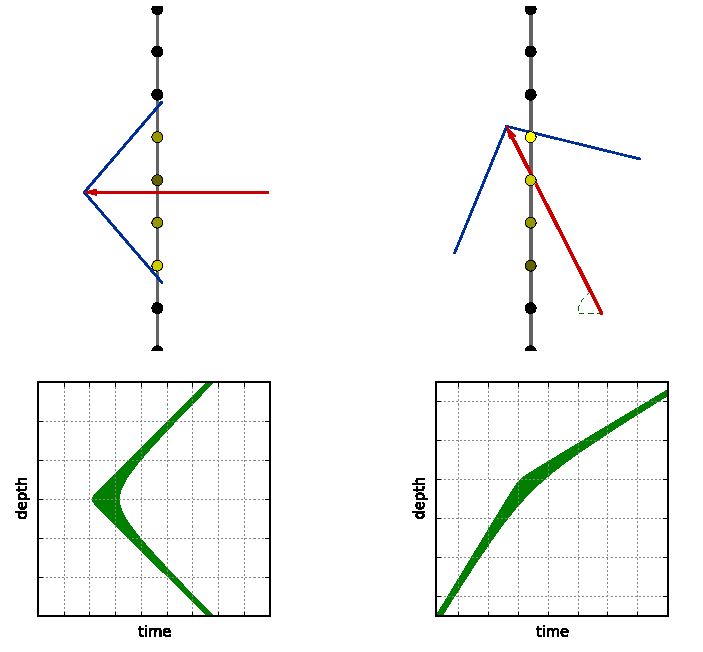
\includegraphics[width=0.8\textwidth]{figures/SANTA_direct_idea.pdf}
	\end{center}
    \caption[Hyperbolic time-depth pattern of muon passing a string, taken from \cite{JPGarza}]
    {Top: Illustrated arrival time differences (dark yellow-early, bright yellow-late) and muon track including Cherenkov light cone (red arrow, blue line).
    Bottom: Hyperbolas formed in time and depth by the direct photons for the two orientations shown in the top. Taken from \cite{JPGarza}.}
    \label{fig:hyperbolic_arrival_time}
\end{figure}

Modeling cascade-like events as isotropic light sources, the arrival time can be obtained by modifying equation \ref{eq:hyperbola_track} and assuming light spreading from the interaction vertex only.
The result also has a hyperbolic shape of the arriving light in time and depth, as described by
\begin{equation}
    t_\gamma(z) = t_0 + \frac{n}{c} \sqrt{d_c^2+(z-z_c)^2},
    \label{eq:hyperbola_cascade}
\end{equation}
where $d_c$ and $z_c$ are depth and distance to the cascade source, respectively.

The equations \ref{eq:hyperbola_track} and \ref{eq:hyperbola_cascade} hold for individual strings, although there is no preferred x-y direction if only one string passed the cleaning procedure.
For those so-called \textit{single-string} events only the zenith angle can be reconstructed and the azimuth has to be obtained by a different reconstruction.
For \textit{multi-string} events, where two or more strings passed the cleaning step, the azimuth angle can also be reconstructed.

The observed time of arrivals are fitted using the modified $\chi^2$ function
\begin{equation}
    \chi^2_{\mathrm{mod}} = \sum_i \Bigg[
        \frac{( t_\gamma(z_i)^{\mathrm{exp}} - t_\gamma(z_i)^{\mathrm{obs}} )^2} {\sigma^2_\gamma} 
        +
        \frac{2 \cdot q(z_i) \cdot \sqrt{r^2_{\mathrm{DOM}}+d^2_\gamma}}{(\cos\phi_\gamma \cdot \bar{q} \cdot d_0)}
    \Bigg],
    \label{eq:chi_squared_santa}
\end{equation}
where $t_\gamma^{\mathrm{exp}/{\mathrm{obs}}}$ are the observed and expected arrival times in the $i$th DOM at depth $z_i$ and $\sigma_\gamma = 3\mathrm{\,ns}$ is the effective time resolution of the DOM.
The additional term in equation \ref{eq:chi_squared_santa} penalizes long photon light paths, since photons traveling short distances are expected to produce the largest signal.
Observing a charge $q(z_i)$ will be disfavored depending on the photon distance $d_\gamma$ traveled to the DOM, with $\bar{q}$ being the mean charge over all selected DOMs, $r_{\mathrm{DOM}}$ the module radius and $\cos\phi_\gamma$ the projected photon arrival angle on the DOM.
$d_0=10\textrm{\,m}$ is a distance that quantifies the strengths of the penalization and it can be understood as the typical distance at which 1\,PE signal is anticipated.


\subsection{Energy Reconstruction} \label{sec:energy_reconstruction}

The neutrino energy is reconstructed in two steps as first described in \cite{Terliuk_masters}.
The steps are based on the previously determined direction of the event.
The position of vertex and endpoint of the track will be re-iteratively modified until the best fit is found.
In the first step, the most probable position, where the muon track has ended, is found by minimizing the logarithm of the likelihood ratio
\begin{equation}
    \mathrm{LLHR} = \mathrm{log}
    \Bigg(
    \frac
    {\prod\limits^{\mathrm{DOMs}}_ip_i(\mathrm{noHit}|\mathrm{Track})}
    {\prod\limits^{\mathrm{DOMs}}_ip_i(\mathrm{noHit}|\mathrm{noTrack})}
    \Bigg)
    ,
    \label{eq:track_no_track_LLLHR}
\end{equation}
with $p_i(\mathrm{noHit}|\mathrm{Track})$ being the probability to see no light if we assume that the muon traveled along an infinite track and $p_i(\mathrm{noHit}|\mathrm{noTrack})$ the probability to see no light assuming a track ending at a certain point.
The products in equation \ref{eq:track_no_track_LLLHR} extend    over all DOMs in a certain radius around the track that do not have seen any light. This procedure is executed as in \cite{SEuler}.
An illustration of the process can be seen in Figure~\ref{fig:finite_reco}.
\begin{figure}[h]
    \centering
      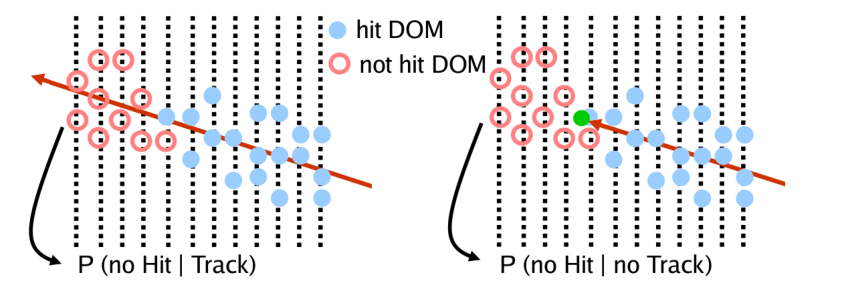
\includegraphics[width=0.8\textwidth]{figures/finiteReco_hitNoHit_track.pdf}
    \caption[Track endpoint reconstruction, taken from \cite{LEERA_internal}]{Visualization showing the track endpoint reconstruction, with the track in red, the endpoint in green, and  the DOMs with signal and without a signal in blue and red, respectively.
    $P_i(\mathrm{noHit}|\mathrm{Track})$ is the probability to see no light for an infinite track and $P_i(\mathrm{noHit}|\mathrm{noTrack})$ the probability to see no light for a finite track.
    Taken from \cite{LEERA_internal}.}
    \label{fig:finite_reco}
\end{figure}
In a second step, the interaction vertex is found using the \textit{hit-no-hit} likelihood with the method presented in \cite{Terliuk_masters} and \cite{LEERA_internal}.
This is done by minimizing the negative logarithmic likelihood 
\begin{equation}
    \mathrm{LLH} = -\sum_i^{\mathrm{DOMs}} \mathrm{log}\,p_i(\lambda_i)
    ,
    \label{eq:hit_no_hit_LLLHR}
\end{equation}
where $p_i(\lambda_i)$ is the probability for a module $i$ to have seen or not to have seen a signal, depending on whether it actually had a signal or not.
The probabilities are calculated with Poisson statistics using
\begin{equation}
    \begin{split}
        p_{\textrm{no-hit}}(\lambda)  & = P_{\textrm{0}}(\lambda) = e^{-\lambda} \textrm{ and } \\
        p_{\textrm{hit}}(\lambda)  & = 1 - P_{\textrm{0}}(\lambda) =  1 - e^{-\lambda},
        \label{eq:poisson_statistics}
    \end{split}
\end{equation}
where $\lambda$ denotes the light expectation. The total light expectation can be estimated with
\begin{equation}
    \lambda = \lambda_\mathrm{track} + \lambda^{\mathrm{1GeV}}_\mathrm{cascade} \cdot   E^{\mathrm{EM}}_\mathrm{cascade} + \nu \cdot \Delta T_\mathrm{event}
    ,
    \label{eq:light_expectations}
\end{equation}
containing the expected number of photons $\lambda_\mathrm{track}$ and $\lambda^{\mathrm{1GeV}}_\mathrm{cascade}$ for a track and for a 1\,GeV cascade, respectively, the EM equivalent energy $E^{\mathrm{EM}}_\mathrm{cascade}$ of the hadronic cascade and the noise rate $\nu$ of the DOM.
The noise rate is scaled with the time duration $T_\mathrm{event}$ of the pulse for the considered event.
The expected number of photons are taken from tables that are based on simulated tracks and electromagnetic cascades at various positions in the detector.
For a given DOM the light expectation of an event located at any point in the detector can be read out from these \textit{photonic} lookup tables \cite{LUNDBERG2007619}.

The total energy of the neutrino is calculated based on the underlying assumption of the occurrence of a hadronic cascade at the interaction point and a muon track originating from this point.
By minimizing the likelihood in equation \ref{eq:hit_no_hit_LLLHR} we find the energy $E^{\mathrm{EM}}_\mathrm{cascade}$ of the hadronic cascade in EM equivalent and the energy of the muon defined by the total length $L_\mu$ of the muon track.
With these quantities and the description of muon energy loss from \cite{GROOM2001183}, the total neutrino energy is given by
\begin{equation}
    E_\nu = \frac{b}{a} (e^{b \cdot L_\mu} - 1) + F^{-1}(E^{\mathrm{EM}}_\mathrm{cascade})
    ,
    \label{eq:total_neutrino_energy}
\end{equation}
where $a=0.266\,\textrm{GeV/m}$ and $b=4.6\cdot 10^{-4}\,\mathrm{m}^{-1}$. The factor $F^{-1}$ accounts for the different amount of light produced by hadronic cascades as compared to electromagnetic cascades.


\section{Event Topologies} \label{sec:event_topologies}

The signals that IceCube detects vary depending on the neutrino flavor and interaction type of the event.
The two main signatures that can be observed are track-like and cascade-like events.
The observed Cherenkov light is produced by the secondary particles originating from the neutrino interactions described in Section~\ref{sec:neutrino_interactions}.
Table~\ref{tab:interactions_vs_signatures} shows an overview of the possible event signatures.
Minimum ionizing muons can travel for long distances and are seen as extended light signatures called tracks.
Muons can come from $\nu_\mu$-CC interactions or from $\nu_\tau$-CC followed by the decay of the $\tau$ to a muon.
However, the $\tau$ only decays to a muon with a branching ratio of BR=17\,\%.

Cascades are the light signal produced by the EM/hadronic showers described in Section~\ref{sec:energy_loss}.
They come from $\nu_e$-CC and most of the $\nu_\tau$-CC interactions because the electron and the tau lose all their energy quickly and only travel a short distance.
They are also produced in all $\nu$-NC interactions since only the hadronic shower is observable and the produced neutrino escapes unseen.
The cascades at the energies considered in this work have a smaller radius than the spacing of the DOMs and are therefore seen as point-like light emitters.

\begin{table}[h]
    \small
    \begin{center}
        \begin{tabular}{  m{2.3cm} m{2.3cm} m{4.5cm} m{3.5cm}  } 
            \hline\hline
            \textbf{Interaction} & \multicolumn{2}{c}{\textbf{Secondary particles}} &\textbf{Signature} \\ 
            \hline\hline
            \multirow{2}{*}[-1.5em]{CC $\overset{\scriptscriptstyle(-)}{\nu_\mu}$ }
            & 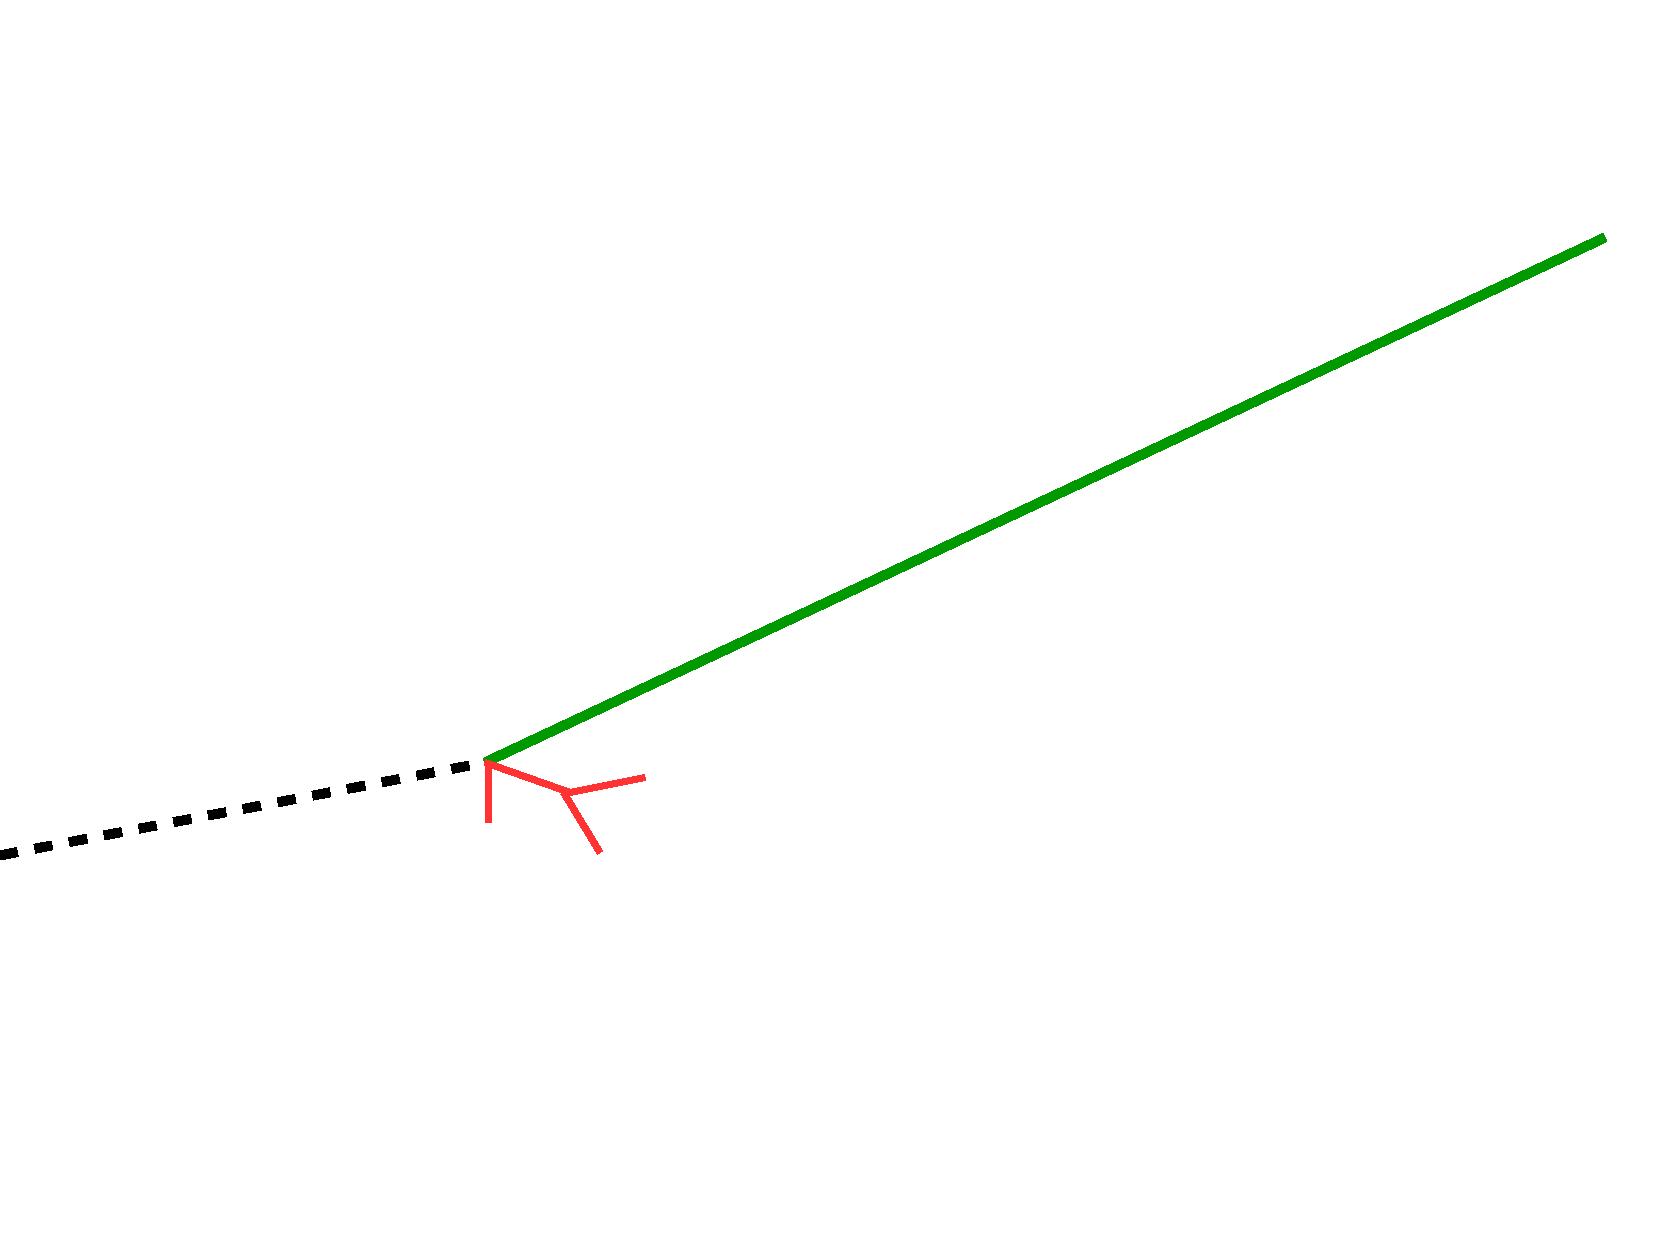
\includegraphics[width=2cm]{figures/numu_CC_muon_only.pdf} 
            & $\mu^\pm$ track 
            & Track-only  \\
            \cmidrule{2-4} 
            &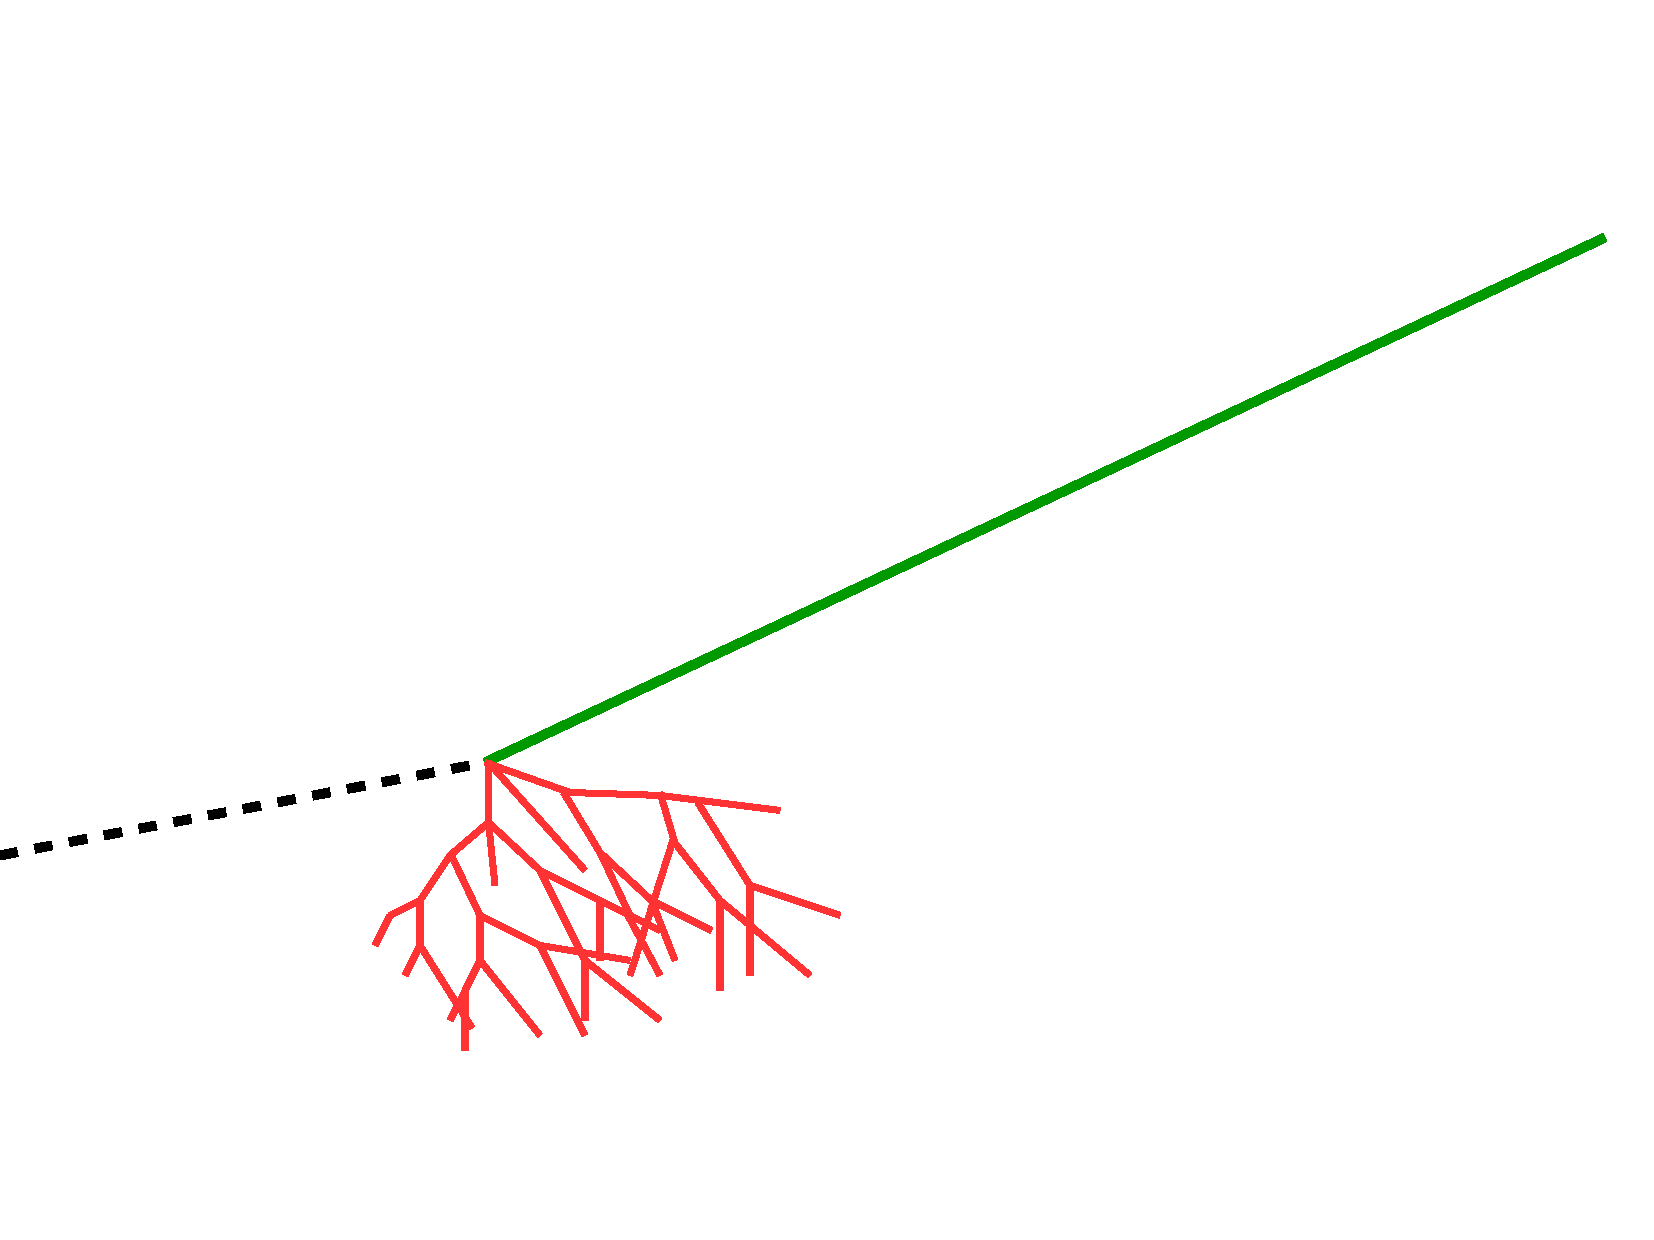
\includegraphics[width=2cm]{figures/numu_CC_track_cascade.pdf}  
            & $\mu^\pm$ track and hadrons 
            & \multirow{2}{*}[-2em]{Track with cascade} \\
            \cmidrule{1-3}
            \multirow{2}{*}[-1.5em]{CC $\overset{\scriptscriptstyle(-)}{\nu_\tau}$ }
            &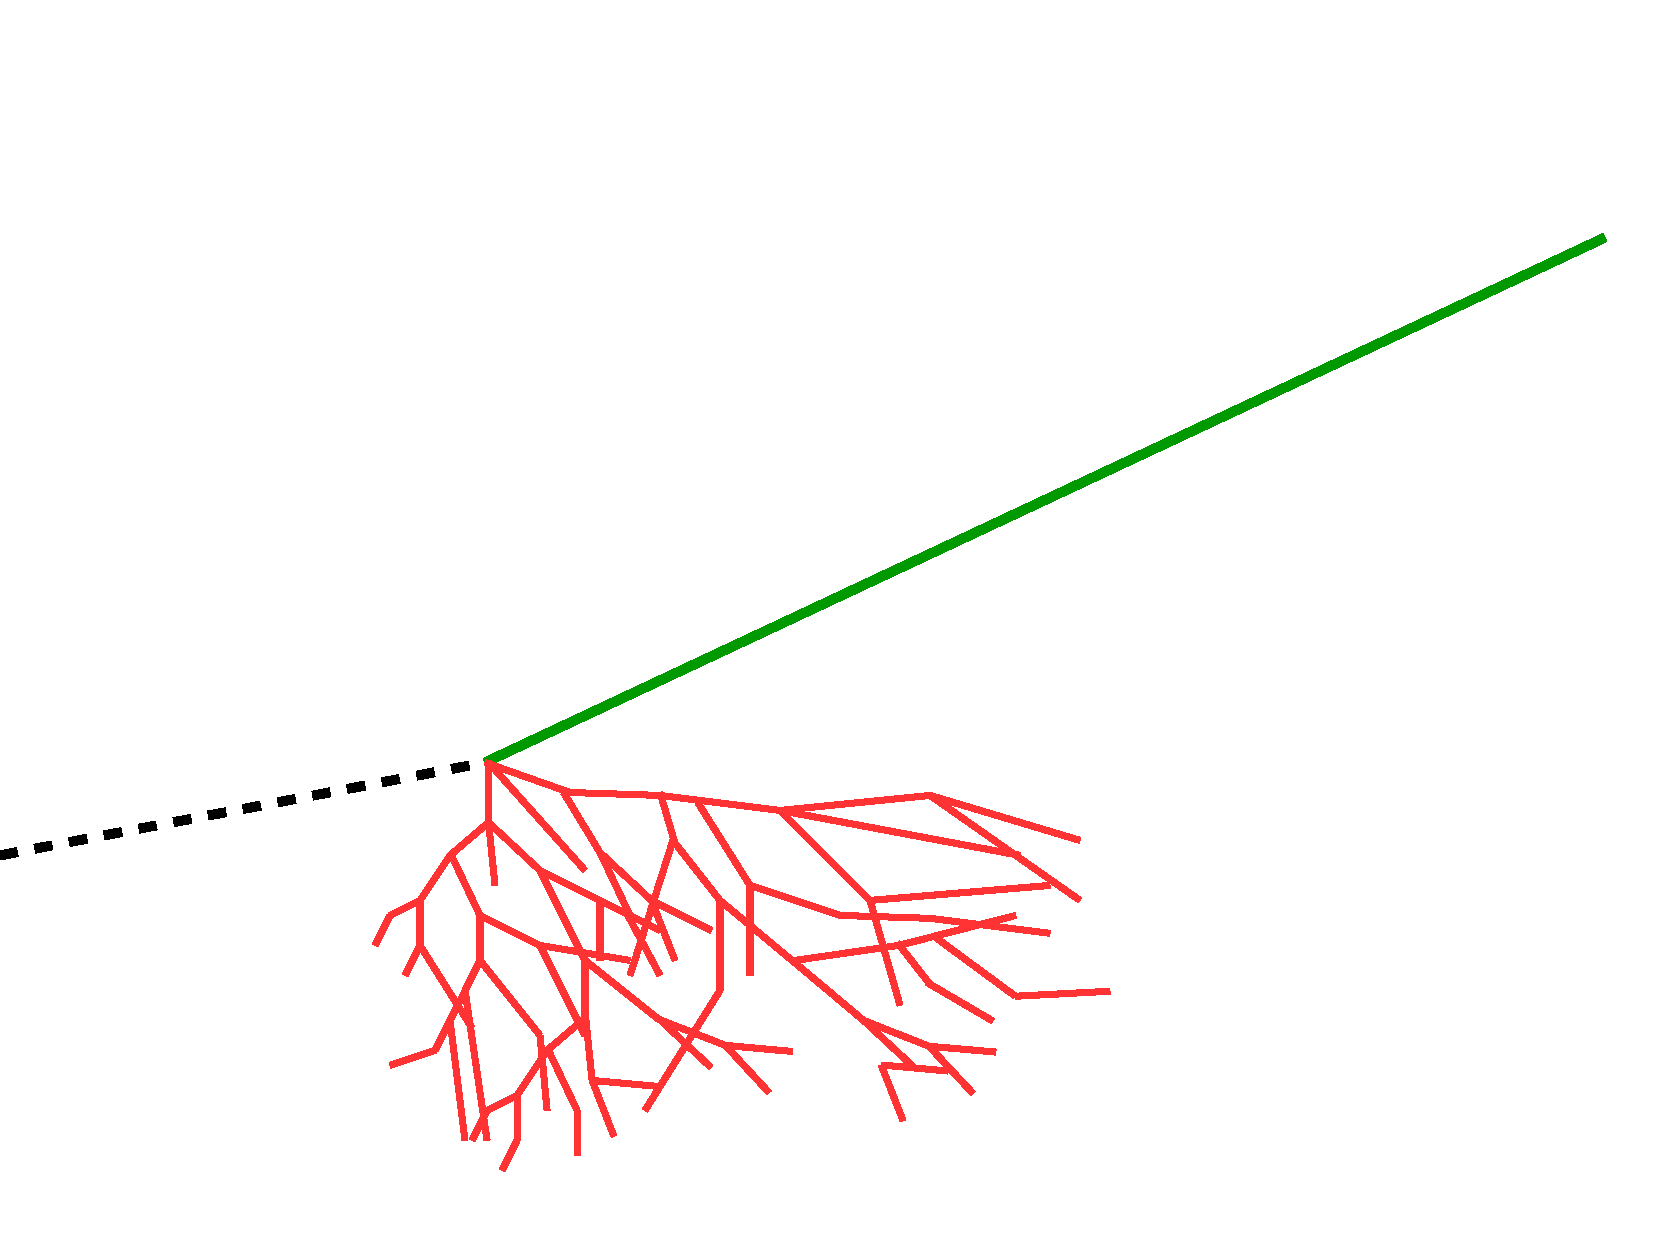
\includegraphics[width=2cm]{figures/nutau_CC_track_cascade.pdf} 
            & $\tau^\pm$ decaying into $\mu^\pm$ ($\sim$17\% BR), hadrons 
            & {}\\
            \cmidrule{2-4}
            & 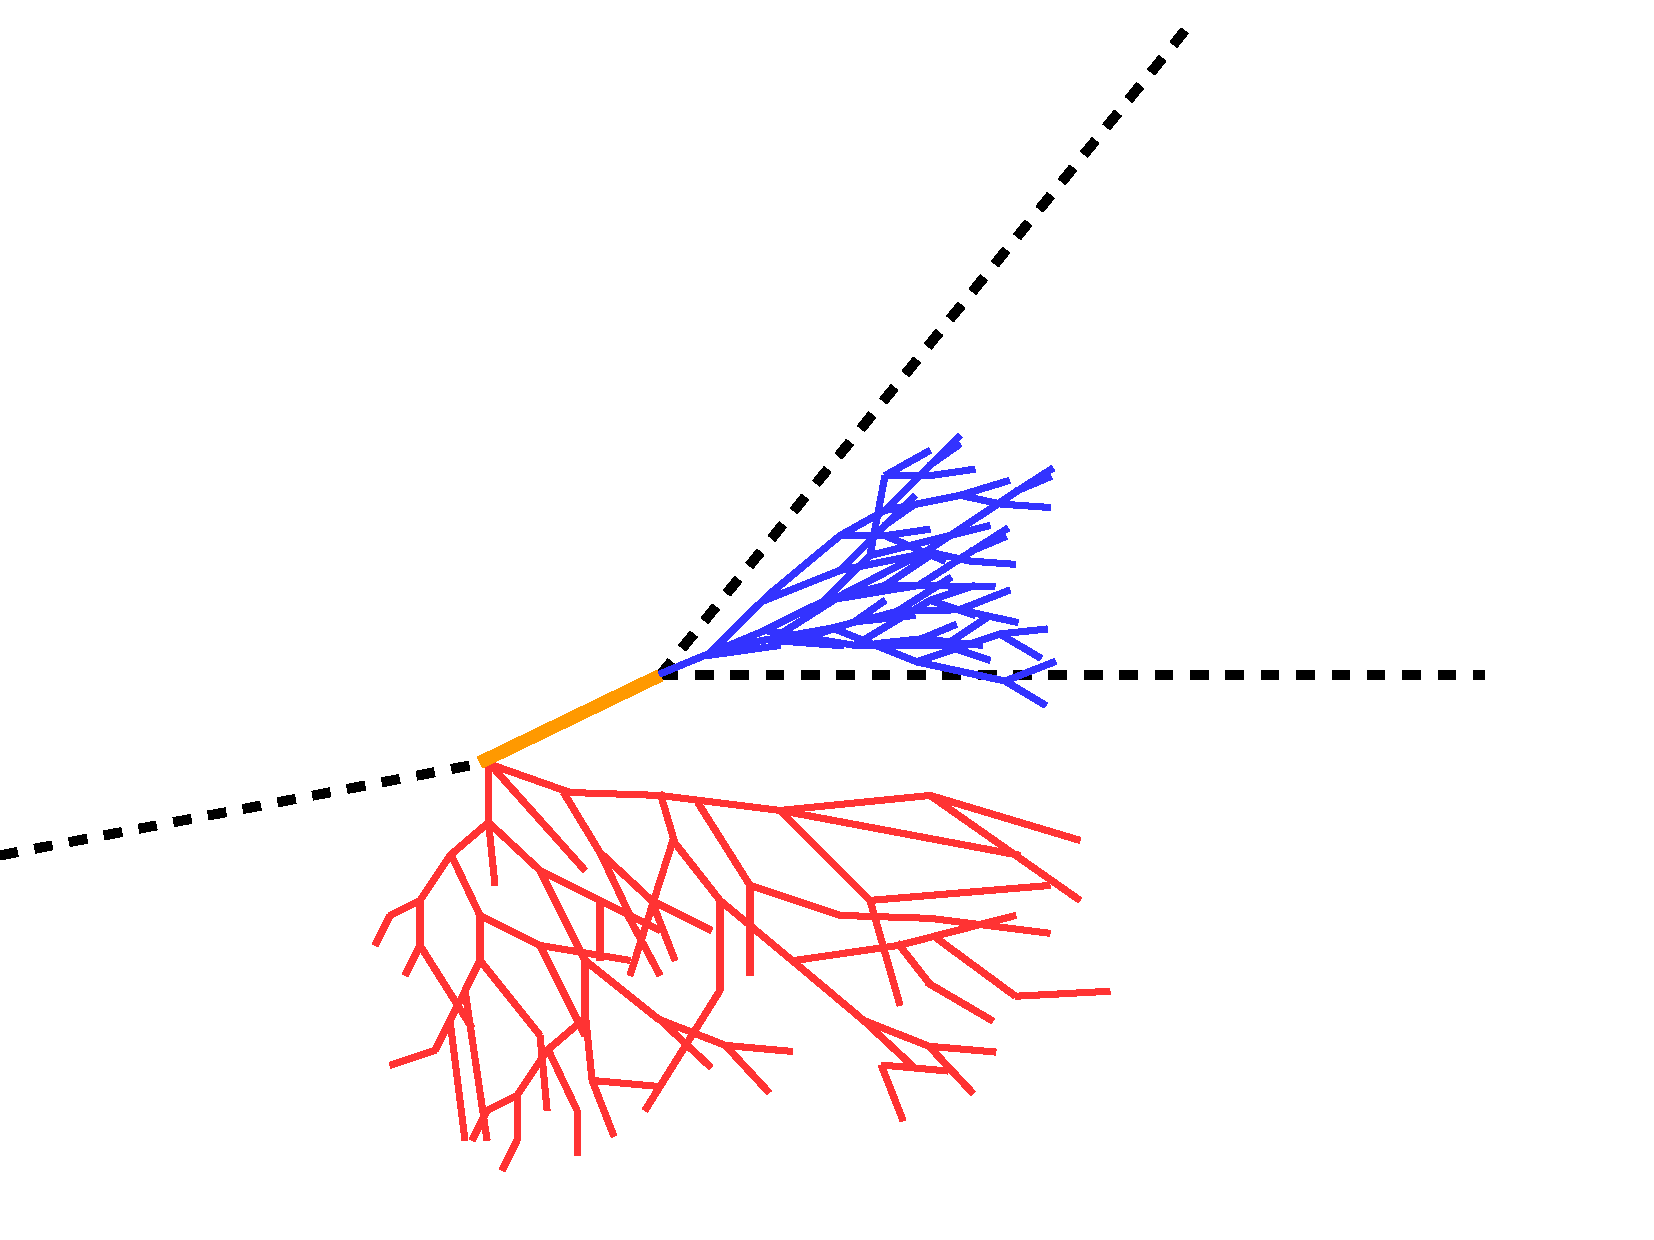
\includegraphics[width=2cm]{figures/nutau_CC_cascadeonly.pdf}
            & $\tau^\pm$ decaying into $e^\pm$ or hadrons ($\sim$83\% BR)  
            & {}\\
            \cmidrule{1-3} CC $\overset{\scriptscriptstyle(-)}{\nu_e}$ 
            & 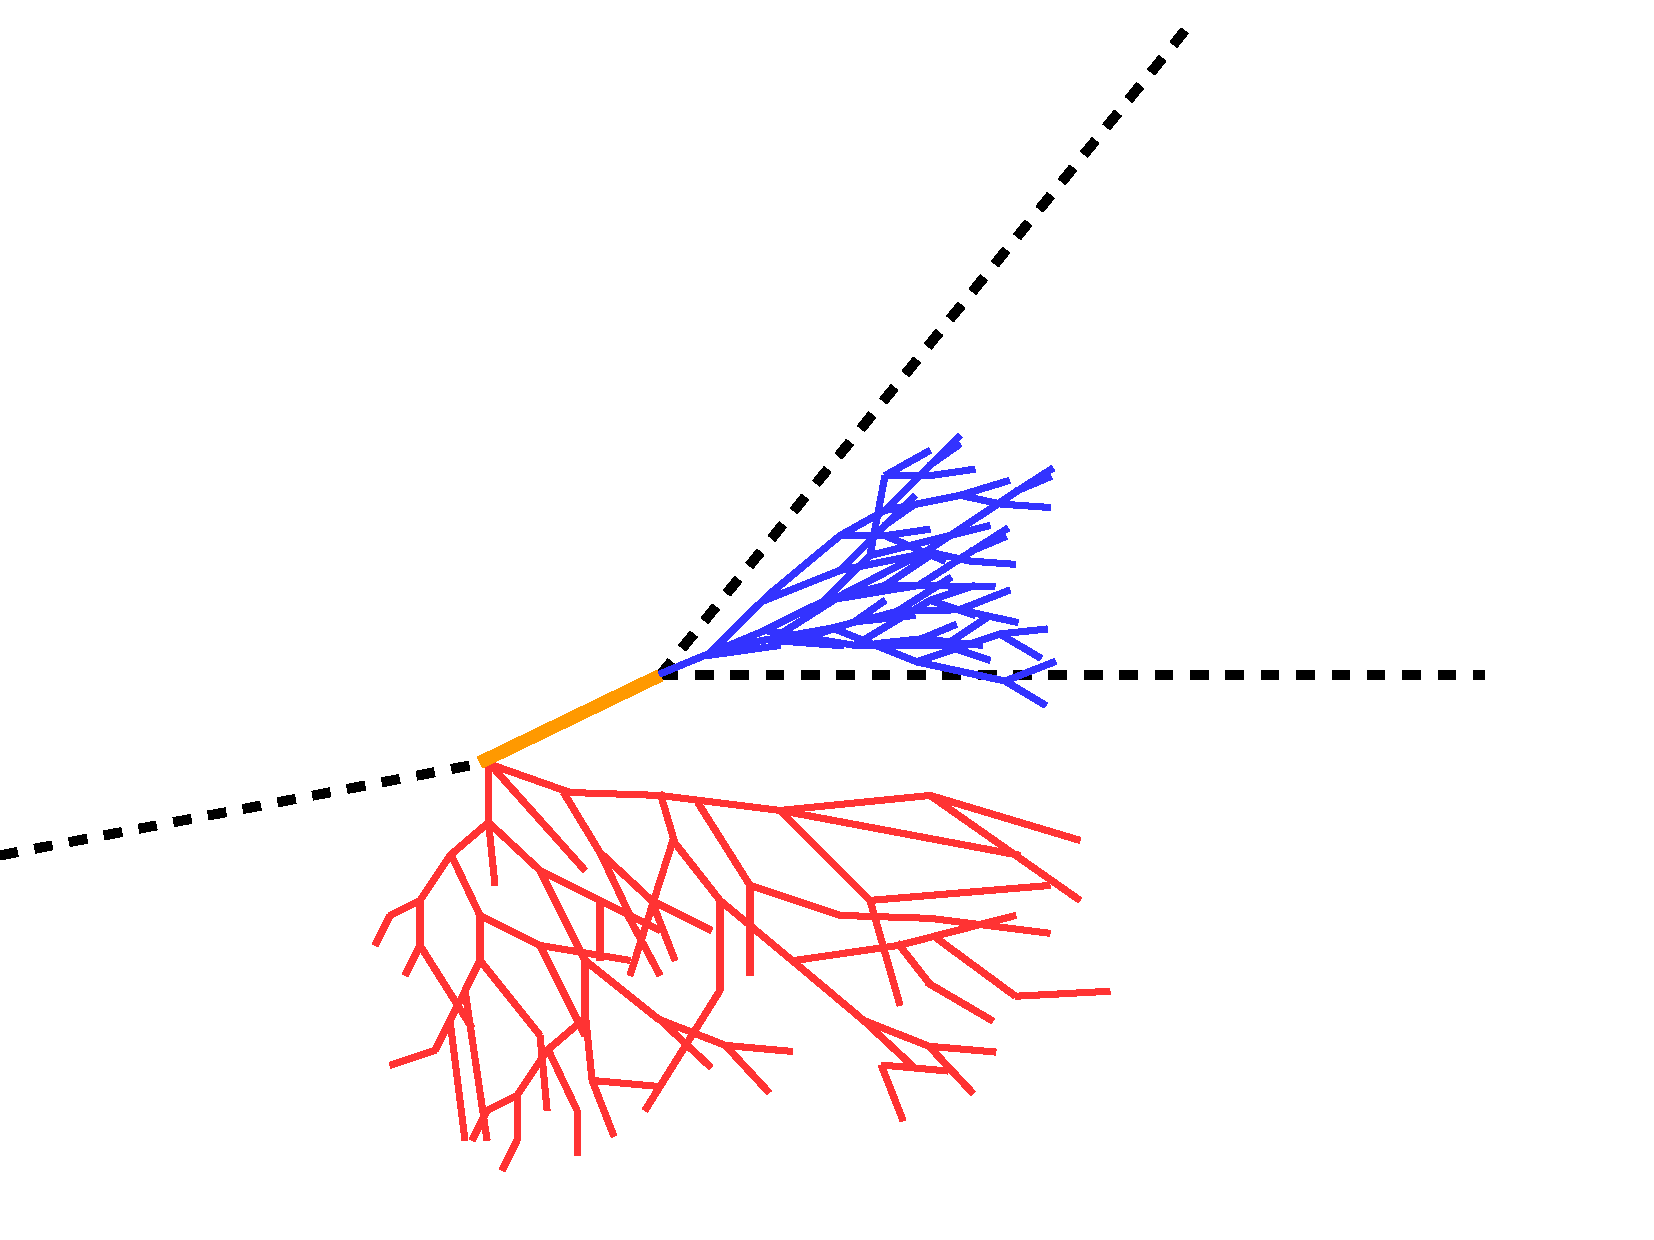
\includegraphics[width=2cm]{figures/nue_CC_cascadeonly.pdf}
            & $e^\pm$, hadrons & {Cascade-only}\\
            \cmidrule{1-3}
            NC $\overset{\scriptscriptstyle(-)}{\nu_\ell}$ 
            & 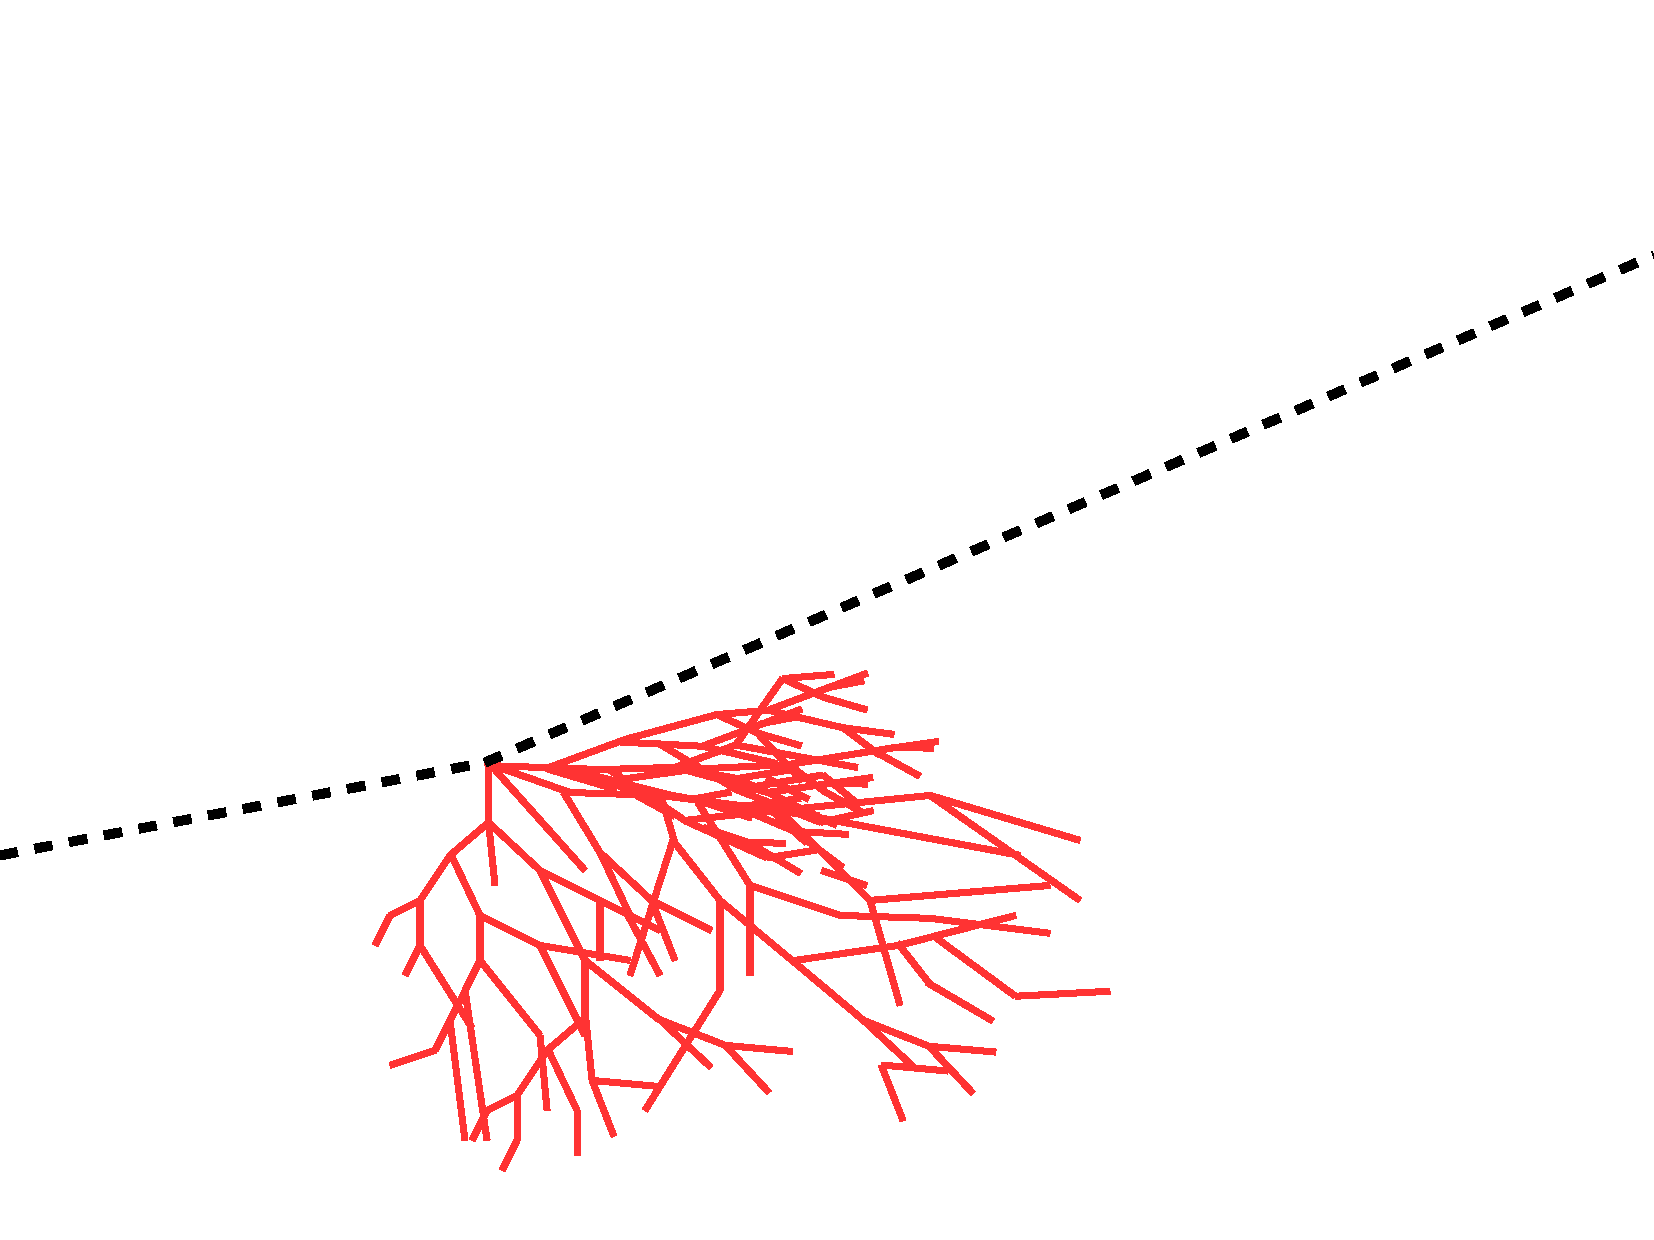
\includegraphics[width=2cm]{figures/nuall_NC_cascadeonly.pdf} 
            & hadrons &  {} \\
            \hline
        \end{tabular}
    \end{center}
    \caption[Event signatures in IceCube and their underlying interactions, taken from~\cite{ATerliuk}]{IceCube event signatures, their underlying interaction type and the particles that produce them. Also shown are the secondary particles produced in the interactions. Black dashed lines represent neutrinos, green lines muons, and blue and red lines are particles in electromagnetic and hadronic cascades, respectively. Taken from~\cite{ATerliuk}.}
    \label{tab:interactions_vs_signatures}
\end{table}

The existence of the two types of event topologies and their origins imply that by identifying track-like events we can identify events coming (mainly) from $\nu_\mu$-CC interactions and therefore obtain a flavor identification.
This is a crucial part of performing an oscillation analysis as will be further discussed in Section~\ref{sec:analysis_principle}.
